\chapter{Geslachtelijke voortplanting van zoogdieren}\label{ch:b2:mammal-reproduction}

Een menselijke eicel is een tiende millimeter groot, de grootste cel van
het lichaam; een zaadcel is een kern met een propeller, een van de
driehonderd miljoen die in één keer worden vrijgelaten, waarvan er enkele
tientallen de eicel zullen bereiken en één haar zal binnendringen. Binnen
een week is de bevruchte eicel een holle bol geworden die zich in de wand
van de baarmoeder ingraaft en uit haar eigen buitenste cellen een orgaan
bouwt --- de \omterm{def:b2:mammal-reproduction:placenta}{placenta} --- waarlangs de moeder haar negen maanden lang zal
voeden. Dan wordt ze geboren en met melk gevoed. Elk zoogdier doet dit;
geen enkel ander dier doet het allemaal. Dit hoofdstuk volgt de gameten
tot de bevruchting, het embryo tot de \omterm{def:b2:mammal-reproduction:implantation}{innesteling}, en het organisme
door dracht, geboorte en lactatie, en eindigt met de manier waarop de
twee geslachten worden gemaakt.

\section{Geslachtsklieren en gameten}

\begin{definition}[De testis en de spermatogenese]\label{def:b2:mammal-reproduction:testis}
\index{spermatogenese}\index{zaadbuisje}\index{sertolicel}\index{leydigcel}
De \emph{testis} is een massa \emph{zaadbuisjes}, samen enkele honderden
meters lang, waarvan de wanden zaadcellen maken; tussen de buisjes liggen
de \emph{leydigcellen}, die testosteron maken. In de wand van het buisje
delen de \emph{spermatogonia} aan de buitenrand zich door mitose, waarbij
ze een stampopulatie in stand houden en cellen naar binnen sturen; die
groeien uit tot primaire \emph{spermatocyten}, die \omterm{def:b2:meiosis-heredity:meiosis}{meiose} I ondergaan (tot
twee secundaire spermatocyten) en \omterm{def:b2:meiosis-heredity:meiosis}{meiose} II (tot vier haploïde
\emph{spermatiden}); de spermatiden stoten het grootste deel van hun
cytoplasma af, condenseren hun kern, vormen een flagel en bedekken de kern
met het \emph{acrosoom}, een blaasje vol enzymen, en worden zo
\emph{spermatozoa} die in het lumen worden vrijgelaten. Grote
\emph{sertolicellen} overspannen de wand, verzorgen de kiemcellen en
vormen met de nauwe verbindingen tussen hen een
\emph{bloed-testisbarrière} die het afweersysteem weghoudt van cellen die
pas in de puberteit verschijnen. De hele reeks duurt bij een man ongeveer
\num{64} dagen en levert van de puberteit tot op hoge leeftijd zo'n
$10^{8}$ zaadcellen per dag op. Zaadcellen verlaten de testis onbeweeglijk
en rijpen twee weken in de \emph{bijbal}.
\end{definition}

\begin{omfigure}
\begin{tikzpicture}[every node/.style={font=\scriptsize}]
  % tubule cross-section: concentric layers
  \draw[thick, fill=omExo!15] (0,0) circle (2.5);
  \draw[thick, fill=omExo!8] (0,0) circle (2.2);
  \draw[thick, fill=omDef!10] (0,0) circle (1.6);
  \draw[thick, fill=omProp!12] (0,0) circle (1.0);
  \draw[thick, fill=white] (0,0) circle (0.45);
  % cells
  \foreach \a in {0,30,...,330} \draw[thick, fill=omDef!40] (\a:2.0) circle (0.13);
  \foreach \a in {15,45,...,345} \draw[thick, fill=omDef!70] (\a:1.32) circle (0.16);
  \foreach \a in {0,20,...,340} \draw[thick, fill=omProp!60] (\a:0.75) circle (0.08);
  \foreach \a in {10,40,...,340} \draw[thick, omProp!80!black] (\a:0.45) -- (\a:0.15);
  % Sertoli cell: tall wedge
  \draw[thick, omExo!70!black, fill=omExo!40, opacity=0.6] (100:2.2) .. controls (90:1.6) and (95:0.9) .. (92:0.5) .. controls (80:0.9) and (75:1.6) .. (72:2.2) -- cycle;
  % Leydig cells outside
  \foreach \p in {(2.9,0.8),(3.1,0.3),(2.8,-0.3)} \draw[thick, fill=omThm!40] \p circle (0.14);
  % labels
  \draw (2.0,0) -- (3.6,-0.5) node[right, align=left] {spermatogonia ($2n$)\\aan de buitenrand};
  \draw (1.32,-0.7) -- (3.6,-1.5) node[right, align=left] {primaire spermatocyten\\(meiose I)};
  \draw (0.75,-0.4) -- (3.6,-2.4) node[right, align=left] {spermatiden ($n$)};
  \draw (0.3,-0.2) -- (3.6,-3.1) node[right, align=left] {spermatozoa in het lumen};
  \draw (2.95,0.55) -- (3.6,0.6) node[right, align=left] {leydigcellen:\\testosteron};
  \draw (88:1.4) -- (3.6,1.8) node[right, align=left] {sertolicel die de wand overspant};
  \node[anchor=east, align=right] at (-2.7,0) {buitenkant\\(basale lamina)};
\end{tikzpicture}

{\small Een \omterm{def:b2:mammal-reproduction:testis}{zaadbuisje} in dwarsdoorsnede. De kiemcellen rijpen van de
buitenwand (spermatogonia) naar binnen (spermatocyten, spermatiden,
spermatozoa in het lumen), ondersteund door sertolicellen; leydigcellen
tussen de buisjes maken testosteron.}
\end{omfigure}

\begin{omfigure}
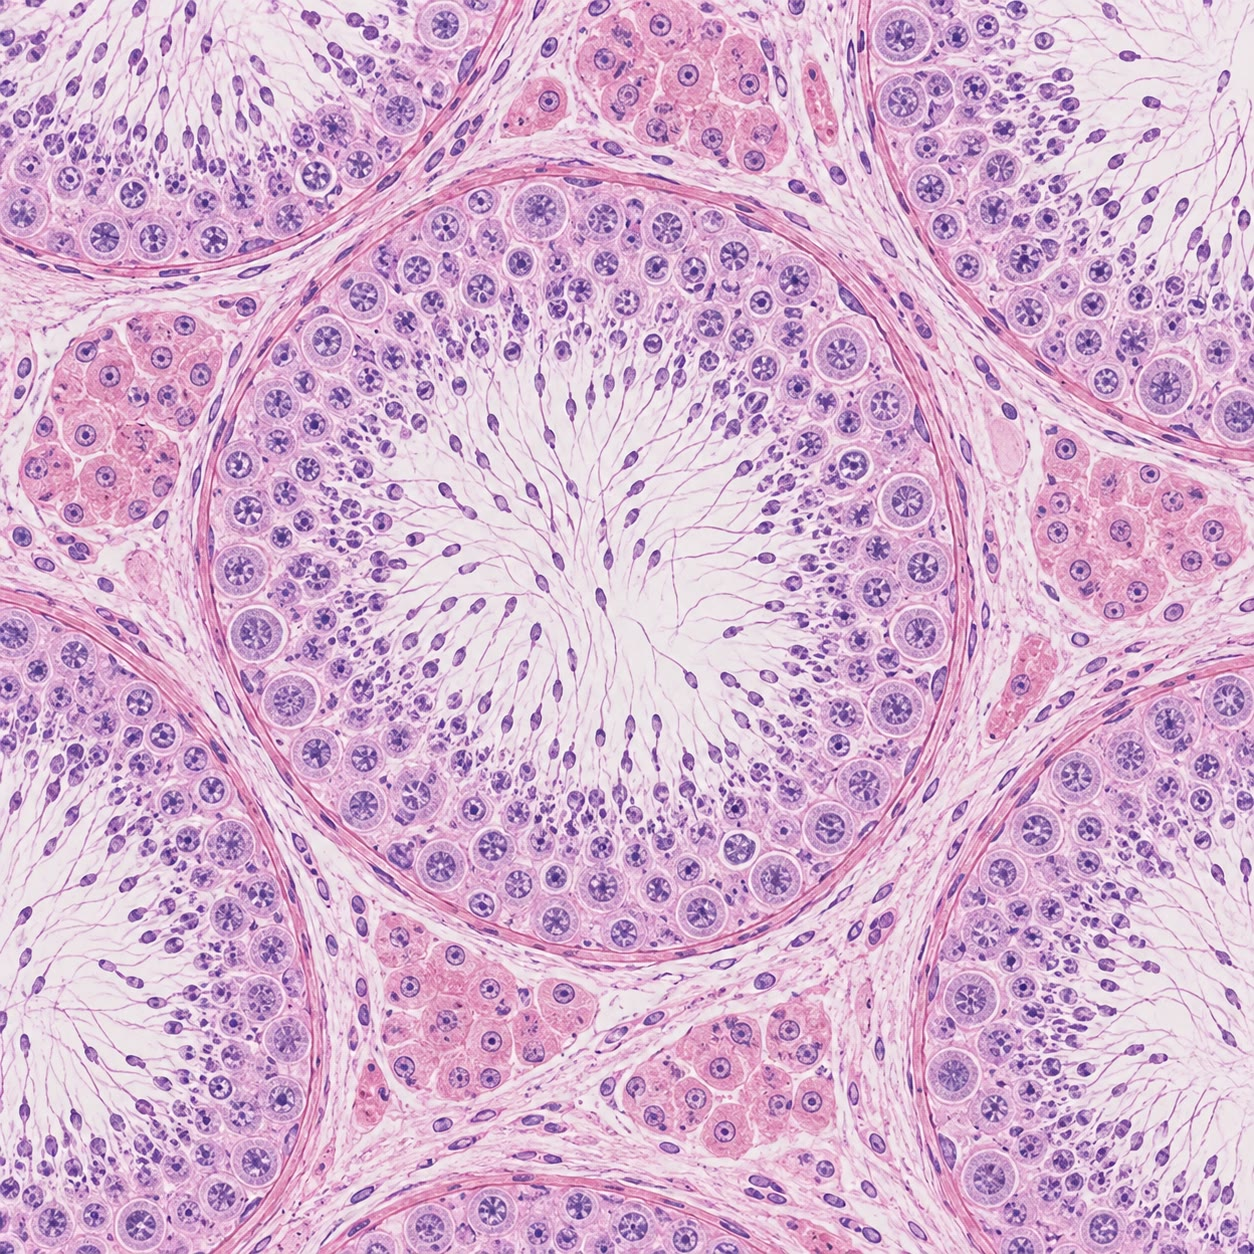
\includegraphics[width=0.42\linewidth]{images/book4/ai/b4-08-testis-histology.jpg}\hspace{0.04\linewidth}
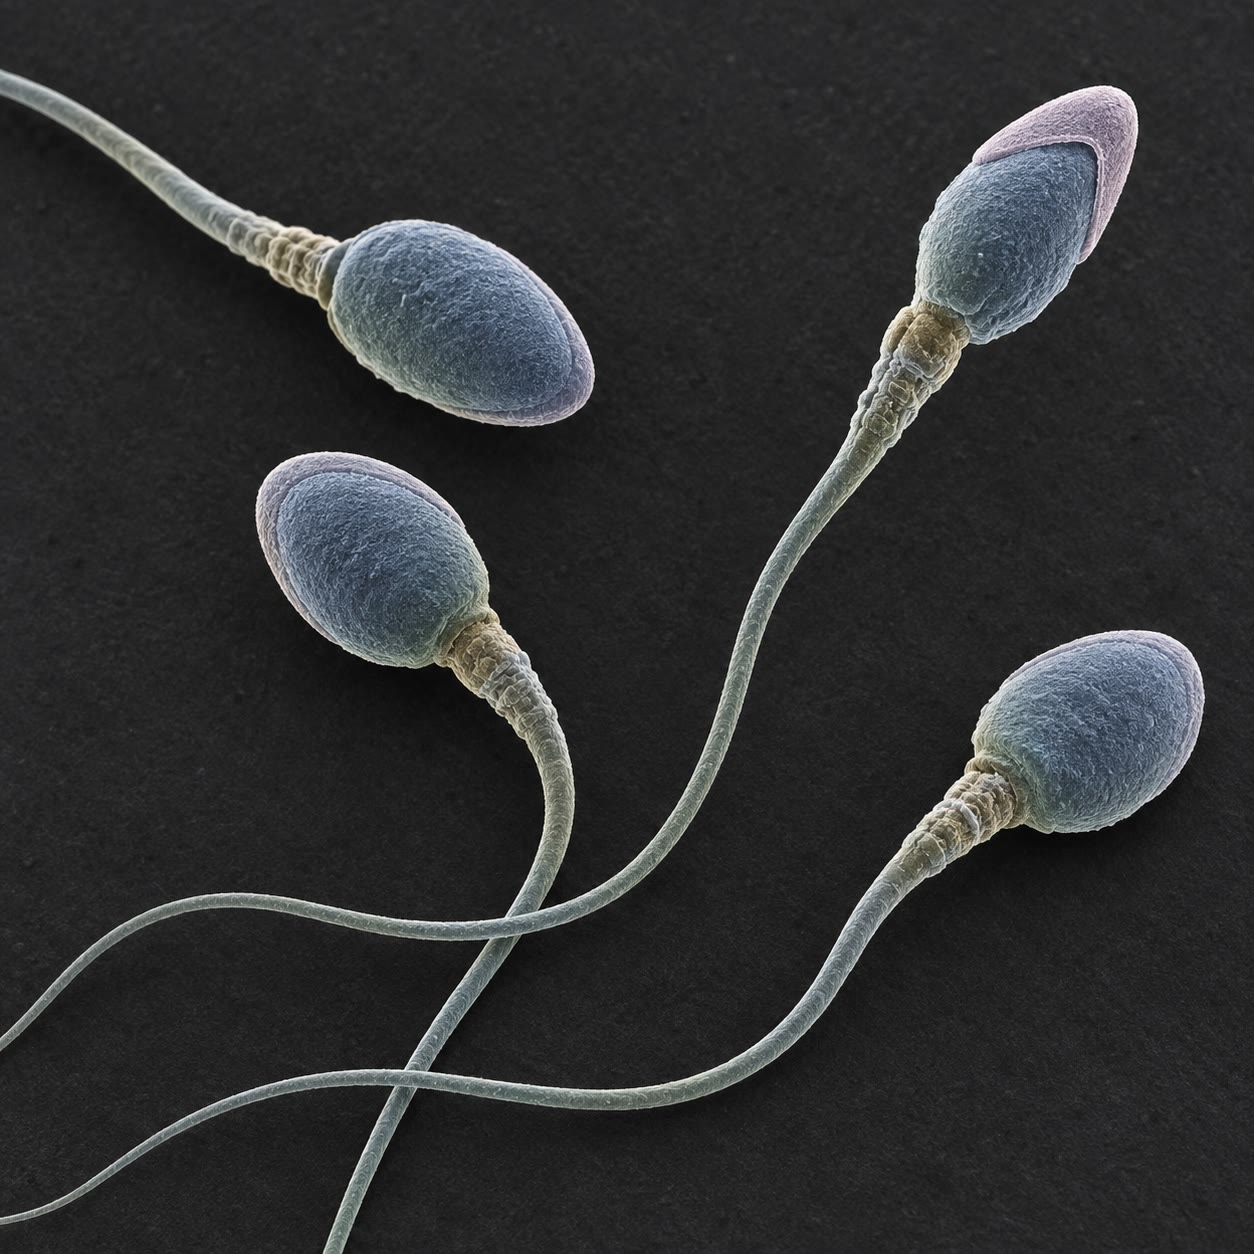
\includegraphics[width=0.42\linewidth]{images/book4/ai/b4-08-sperm-sem.jpg}

{\small Links: \omterm{def:b2:mammal-reproduction:testis}{zaadbuisjes} in doorsnede, met de kiemcellen gelaagd van de
wand tot het lumen. Rechts: spermatozoa onder de
rasterelektronenmicroscoop, met het acrosoomkapje zichtbaar op de koppen.}
\end{omfigure}

\begin{definition}[Het ovarium en de oögenese]\label{def:b2:mammal-reproduction:ovary}
\index{oögenese}\index{follikel}\index{ovulatie}\index{corpus luteum}
De oögenese is in bijna elk opzicht het spiegelbeeld van de
\omterm{def:b2:mammal-reproduction:testis}{spermatogenese}. De \emph{oögonia} vermenigvuldigen zich alleen bij de
foetus: bij de geboorte draagt een meisje een voorraad van ongeveer een
miljoen primaire \emph{oöcyten}, elk gestopt in \omterm{prop:b2:meiosis-heredity:stages}{profase I} van de \omterm{def:b2:meiosis-heredity:meiosis}{meiose} en
omhuld door één laag cellen --- een \emph{primordiale follikel} --- en er
worden nooit nieuwe gemaakt. Vanaf de puberteit groeit elke maand een
cohort follikels: de oöcyt wordt groter, de omringende
\emph{granulosacellen} vermenigvuldigen zich tot lagen, een buitenste
\emph{theca} vormt zich, een met vocht gevulde holte gaat open (de
\emph{follikel van De Graaf}, twee centimeter groot), en meestal bereikt
er één de \emph{ovulatie}: de oöcyt, die pas nu \omterm{def:b2:meiosis-heredity:meiosis}{meiose} I voltooit en
opnieuw stopt in metafase II, wordt met zijn krans van granulosacellen in
de eileider uitgestoten. De lege follikel wordt het \emph{corpus luteum},
een tijdelijke klier die progesteron maakt. De \omterm{def:b2:meiosis-heredity:meiosis}{meiose} levert één eicel en
drie piepkleine poollichaampjes op --- al het cytoplasma gaat naar één cel
--- en \omterm{def:b2:meiosis-heredity:meiosis}{meiose} II wordt pas voltooid als er een zaadcel binnendringt. Van de
miljoen oöcyten worden er in een leven ongeveer \num{400} geovuleerd; de
rest degenereert (\emph{atresie}), en wanneer de voorraad rond de
vijftig is uitgeput, stoppen de cycli: de menopauze.
\end{definition}

\begin{omfigure}
\begin{tikzpicture}[every node/.style={font=\scriptsize}, >=stealth]
  % timeline of oogenesis vs spermatogenesis
  \draw[thick, ->] (0,3.0) -- (12.6,3.0); \node[anchor=west] at (12.6,3.0) {leeftijd};
  \foreach \x/\l in {0/{foetus}, 2.2/{geboorte}, 4.6/{puberteit}, 10.2/{$\sim$50 jaar}}
    \draw (\x,3.1) -- (\x,2.9) node[above=0.15cm] {\l};
  % oogenesis line
  \node[anchor=east, omThm] at (-0.2,1.5) {oögenese};
  \draw[very thick, omThm] (0,1.5) -- (1.6,1.5); \node[above, omThm, align=center] at (0.8,1.55) {oögonia\\vermenigvuldigen};
  \draw[very thick, omThm, dashed] (1.6,1.5) -- (4.6,1.5); \node[below, omThm] at (3.1,1.45) {stilstand in profase I};
  \draw[very thick, omThm] (4.6,1.5) -- (10.2,1.5); \node[above, omThm, align=center] at (7.4,1.55) {één ovulatie per maand;\\meiose I voltooid bij ovulatie, II bij bevruchting};
  \fill[omThm] (10.2,1.5) circle (0.07); \node[below, omThm] at (10.2,1.45) {voorraad uitgeput};
  % spermatogenesis line
  \node[anchor=east, omDef] at (-0.2,0.3) {spermatogenese};
  \draw[very thick, omDef, dashed] (0,0.3) -- (4.6,0.3); \node[above, omDef] at (2.3,0.35) {spermatogonia in rust};
  \draw[very thick, omDef, ->] (4.6,0.3) -- (12.6,0.3); \node[above, omDef] at (8.6,0.35) {continu: $10^{8}$ zaadcellen per dag, elk 64 dagen, uit stamcellen};
\end{tikzpicture}

{\small De twee gametogeneses in de tijd. Oöcyten worden alle vóór de
geboorte gemaakt en een voor een uit een eindige voorraad vrijgelaten;
zaadcellen worden het hele volwassen leven lang continu uit stamcellen
gemaakt.}
\end{omfigure}

\begin{omfigure}
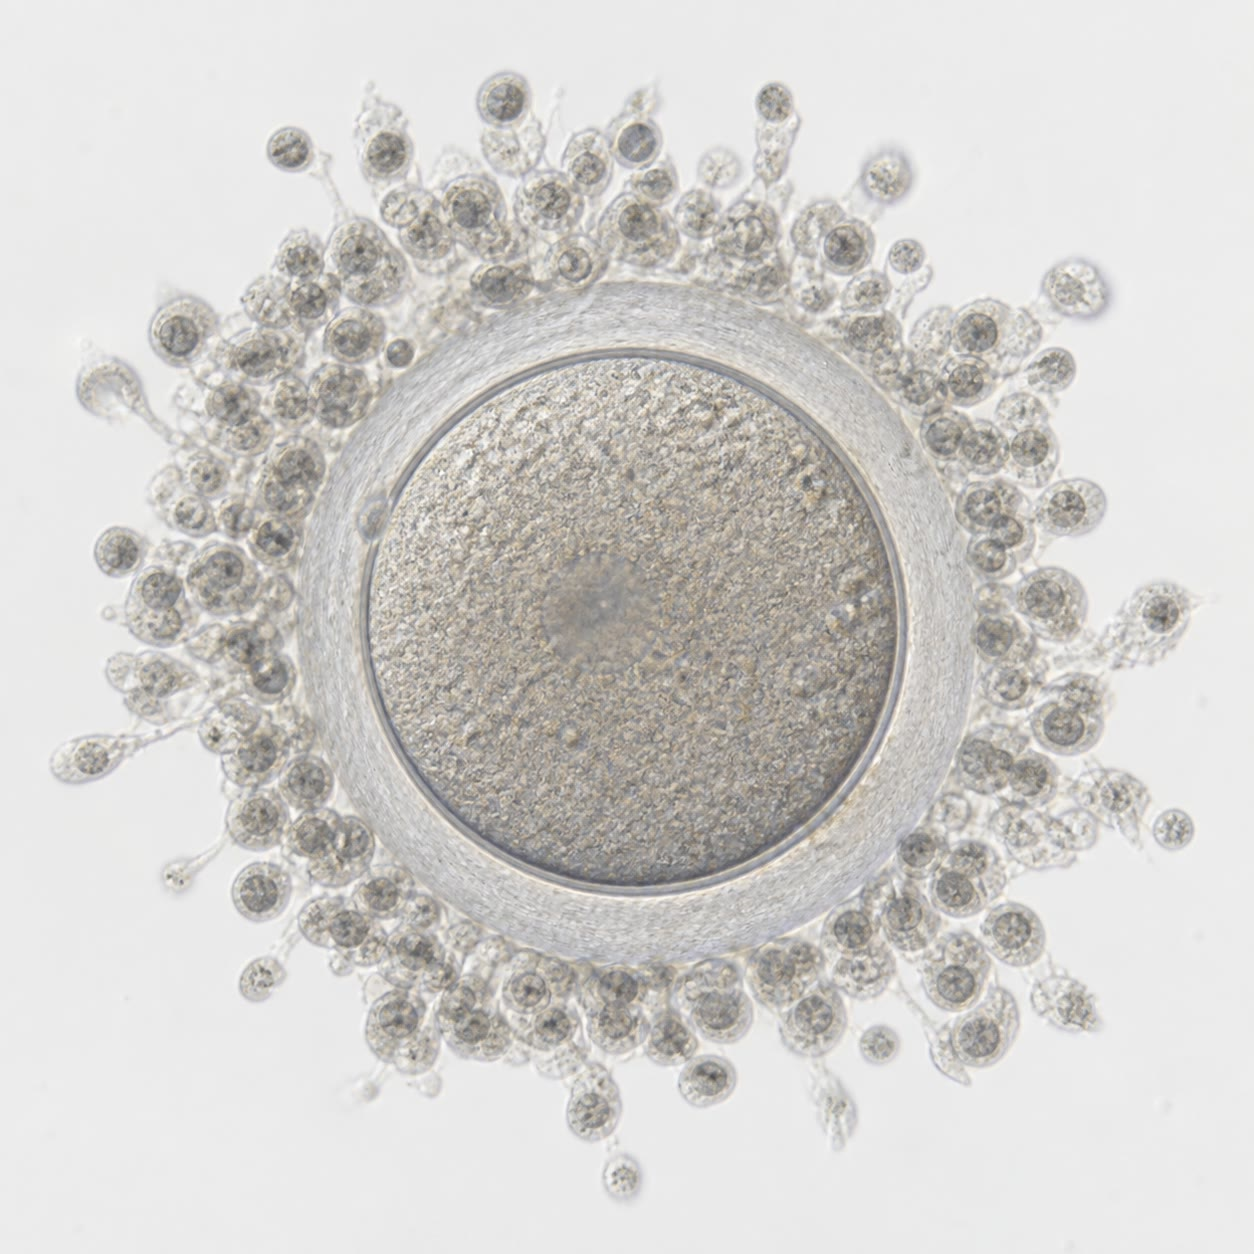
\includegraphics[width=0.46\linewidth]{images/book4/ai/b4-08-oocyte.jpg}

{\small Een geovuleerde oöcyt: de cel, haar doorzichtige mantel (de \omterm{prop:b2:mammal-reproduction:fertilisation}{zona
pellucida}), en de wolk granulosacellen die met haar de \omterm{def:b2:mammal-reproduction:ovary}{follikel} verliet.}
\end{omfigure}

\section{Bevruchting}

\begin{proposition}[De stappen van de bevruchting]\label{prop:b2:mammal-reproduction:fertilisation}
\index{bevruchting!bij zoogdieren}\index{acrosoomreactie}\index{zona pellucida}\index{corticale reactie}
Zaadcellen die in de vagina worden afgezet --- zo'n $3\times 10^{8}$ ---
steken het slijm van de baarmoederhals over, worden door de samentrekkingen
van de baarmoeder omhoog gevoerd, en enkele honderden bereiken binnen een
uur de ampulla van de eileider, waar de eicel een dag wacht. Onderweg
ondergaan de zaadcellen \emph{capacitatie}: secreties van het
vrouwelijke kanaal ontdoen hun membranen van bedekkende eiwitten en maken
ze hyperactief. Bij de eicel dringt een zaadcel door de granulosacellen,
bindt aan een glycoproteïne van de \emph{\omterm{prop:b2:mammal-reproduction:fertilisation}{zona pellucida}}, en ondergaat de
\emph{acrosoomreactie}, waarbij enzymen vrijkomen die een weg door de zona
verteren; haar membraan versmelt met dat van de eicel, en de kern van de
zaadcel gaat naar binnen. De eicel reageert binnen seconden: calcium
golft door haar heen, en corticale korrels geven enzymen af die de zona
verharden en haar receptoren voor zaadcellen verwijderen --- de
\emph{\omterm{prop:b2:mammal-reproduction:fertilisation}{corticale reactie}}, de blokkade van polyspermie.
De eicel voltooit \omterm{def:b2:meiosis-heredity:meiosis}{meiose} II, stoot het tweede poollichaampje af, en de
twee haploïde \emph{pronuclei} repliceren hun DNA, komen samen en gaan de
eerste mitose in: de zygote is een dag oud. De soortspecificiteit ligt in
de eiwitten van de zona, en daarom dringt een zaadcel van een muis een
menselijke eicel niet binnen.
\end{proposition}
\begin{proof}[Bewijsmateriaal]
Edwards en Steptoe (1978) bevruchtten een menselijke oöcyt, kort voor de
\omterm{def:b2:mammal-reproduction:ovary}{ovulatie} uit het ovarium gehaald, in een schaaltje met gecapaciteerde
zaadcellen, kweekten het embryo tot acht cellen en brachten het terug in
de baarmoeder, waar het zich innestelde en werd geboren: in-vitrofertilisatie.
Elke stap van de bovenstaande reeks was eerst uitgewerkt bij de zee-egel en
de muis, waar de versmelting, de calciumgolf en het vrijkomen van de
corticale korrels kunnen worden bekeken; bij de muis levert het
wegnemen van één glycoproteïne van de zona (ZP2 of ZP3) door \omterm{def:b2:genome-diversification:mutation}{mutatie}
eicellen op waaraan zaadcellen niet kunnen binden.
\end{proof}

\begin{theorem}[Waarom één eicel miljoenen zaadcellen nodig heeft]\label{thm:b2:mammal-reproduction:poisson}
\index{polyspermie}
Als van de $N$ afgezette zaadcellen elke zaadcel onafhankelijk met een
kleine kans $\pi$ het oppervlak van de eicel bereikt, is het aantal dat
aankomt poissonverdeeld met gemiddelde $m = N\pi$ en is de kans dat er
minstens één aankomt
\[
P = 1 - e^{-m}.
\]
Met $N = 3\times 10^{8}$ en $\pi \approx 10^{-8}$ is $m \approx 3$
en $P \approx 0.95$; met $N = 2\times 10^{7}$ (de klinische drempel van
een laag aantal zaadcellen) is $m = 0.2$ en $P = 0.18$. Dezelfde
rekensom laat zien waarom de blokkade van polyspermie onmisbaar is:
wanneer
$P$ hoog is, komen er binnen enkele seconden meerdere zaadcellen aan, en
een eicel waarin er twee binnendringen, zou triploïd zijn en sterven.
\end{theorem}
\begin{proof}
Elke zaadcel is een onafhankelijk experiment met succeskans $\pi$;
het aantal successen is binomiaal verdeeld, wat voor grote $N$ en kleine
$\pi$ een poissonverdeling met gemiddelde $N\pi$ is. De kans op nul
successen is $e^{-m}$, dus op minstens één $1 - e^{-m}$; de
kans op twee of meer is $1 - e^{-m}(1 + m)$, ongeveer $0.8$ voor
$m = 3$.
\end{proof}

\begin{omfigure}
\begin{tikzpicture}[every node/.style={font=\scriptsize}, >=stealth]
  \foreach \x/\lab in {0/{1. zaadcel bindt\\aan de zona}, 3.3/{2. acrosoomreactie:\\enzymen banen een weg}, 6.6/{3. membranen versmelten;\\calciumgolf}, 9.9/{4. corticale reactie:\\zona verhard,\\meiose II voltooid}} {
    \begin{scope}[xshift=\x cm]
      \draw[thick, fill=omThm!8] (0,0) circle (0.9);
      \draw[thick, omExo!70!black] (0,0) circle (1.15);
      \node[below, align=center] at (0,-1.3) {\lab};
    \end{scope}
  }
  % stage 1: sperm at zona
  \draw[thick, fill=omDef!50] (-1.45,0.1) ellipse (0.18 and 0.11); \draw[thick, omDef] (-1.63,0.1) .. controls (-2.0,0.4) and (-2.2,-0.2) .. (-2.5,0.1);
  % stage 2: sperm digging through zona
  \begin{scope}[xshift=3.3cm]
    \fill[white] (-1.2,0.0) circle (0.12);
    \draw[thick, fill=omDef!50] (-1.05,0.05) ellipse (0.18 and 0.11); \draw[thick, omDef] (-1.23,0.05) .. controls (-1.6,0.35) and (-1.8,-0.25) .. (-2.1,0.05);
    \foreach \a in {150,170,190,210} \draw[omProp, thick] (-1.2,0.0) -- ++(\a:0.25);
  \end{scope}
  % stage 3: fused, calcium wave
  \begin{scope}[xshift=6.6cm]
    \fill[white] (-1.15,0.0) circle (0.12);
    \draw[thick, fill=omDef!50] (-0.75,0.0) ellipse (0.18 and 0.11);
    \draw[thick, omDef] (-0.93,0.0) .. controls (-1.3,0.3) and (-1.5,-0.3) .. (-1.8,0.0);
    \foreach \r in {0.35,0.55,0.75} \draw[omProp, thick] (-0.75,0) ++(-60:\r) arc (-60:60:\r);
  \end{scope}
  % stage 4: hardened zona, polar body, pronuclei
  \begin{scope}[xshift=9.9cm]
    \draw[very thick, omExo!70!black] (0,0) circle (1.15);
    \draw[thick, fill=omDef!30] (-0.25,0.05) circle (0.2); \draw[thick, fill=omThm!30] (0.25,0.05) circle (0.2);
    \draw[thick, fill=omThm!20] (0.55,0.95) circle (0.12);
    \node[anchor=west] at (1.2,0.9) {poollichaampje};
    \draw (0.45,0.05) -- (1.2,-0.35); \node[anchor=west] at (1.2,-0.35) {twee pronuclei};
  \end{scope}
\end{tikzpicture}

{\small Bevruchting in vier stappen: binding aan de zona, de
acrosoomreactie, versmelting en de calciumgolf, en de \omterm{prop:b2:mammal-reproduction:fertilisation}{corticale reactie}
die de eicel voor andere zaadcellen afsluit terwijl ze de \omterm{def:b2:meiosis-heredity:meiosis}{meiose}
voltooit.}
\end{omfigure}

\section{Innesteling en de placenta}

\begin{definition}[Klieving, blastocyste, innesteling]\label{def:b2:mammal-reproduction:implantation}
\index{blastocyste}\index{trofoblast}\index{binnenste celmassa}\index{innesteling}
De zygote deelt zich om de twaalf tot twintig uur zonder te groeien
(\emph{klieving}) terwijl ze door de eileider omlaag wordt gevoerd: twee
cellen, vier, acht, een compacte bol van zestien (\emph{morula}), en tegen
dag vijf een \emph{blastocyste} van ongeveer honderd cellen: een buitenste
laag, de \emph{trofoblast}, rond een holte, met aan één kant een klompje
cellen, de \emph{binnenste celmassa}. De trofoblast zal de \omterm{def:b2:mammal-reproduction:placenta}{placenta} en de
vliezen bouwen; de binnenste celmassa wordt het embryo --- en levert, in
dit stadium weggenomen, embryonale stamcellen op. Op dag zes komt de
blastocyste uit haar zona, hecht zich aan het slijmvlies van de
baarmoeder, en dringt de trofoblast erin binnen: cellen versmelten tot een
meerkernig front dat maternaal weefsel verteert en maternale haarvaten
opent, zodat het embryo tegen dag twaalf in de wand is begraven en in
maternaal bloed baadt. Dit is de \emph{innesteling}. Ze slaagt alleen in
een baarmoeder die door progesteron is voorbereid, binnen een venster van
enkele dagen; ongeveer de helft van alle menselijke conceptussen gaat vóór
of bij deze stap verloren, meestal door chromosoomfouten van de eicel.
\end{definition}

\begin{omfigure}
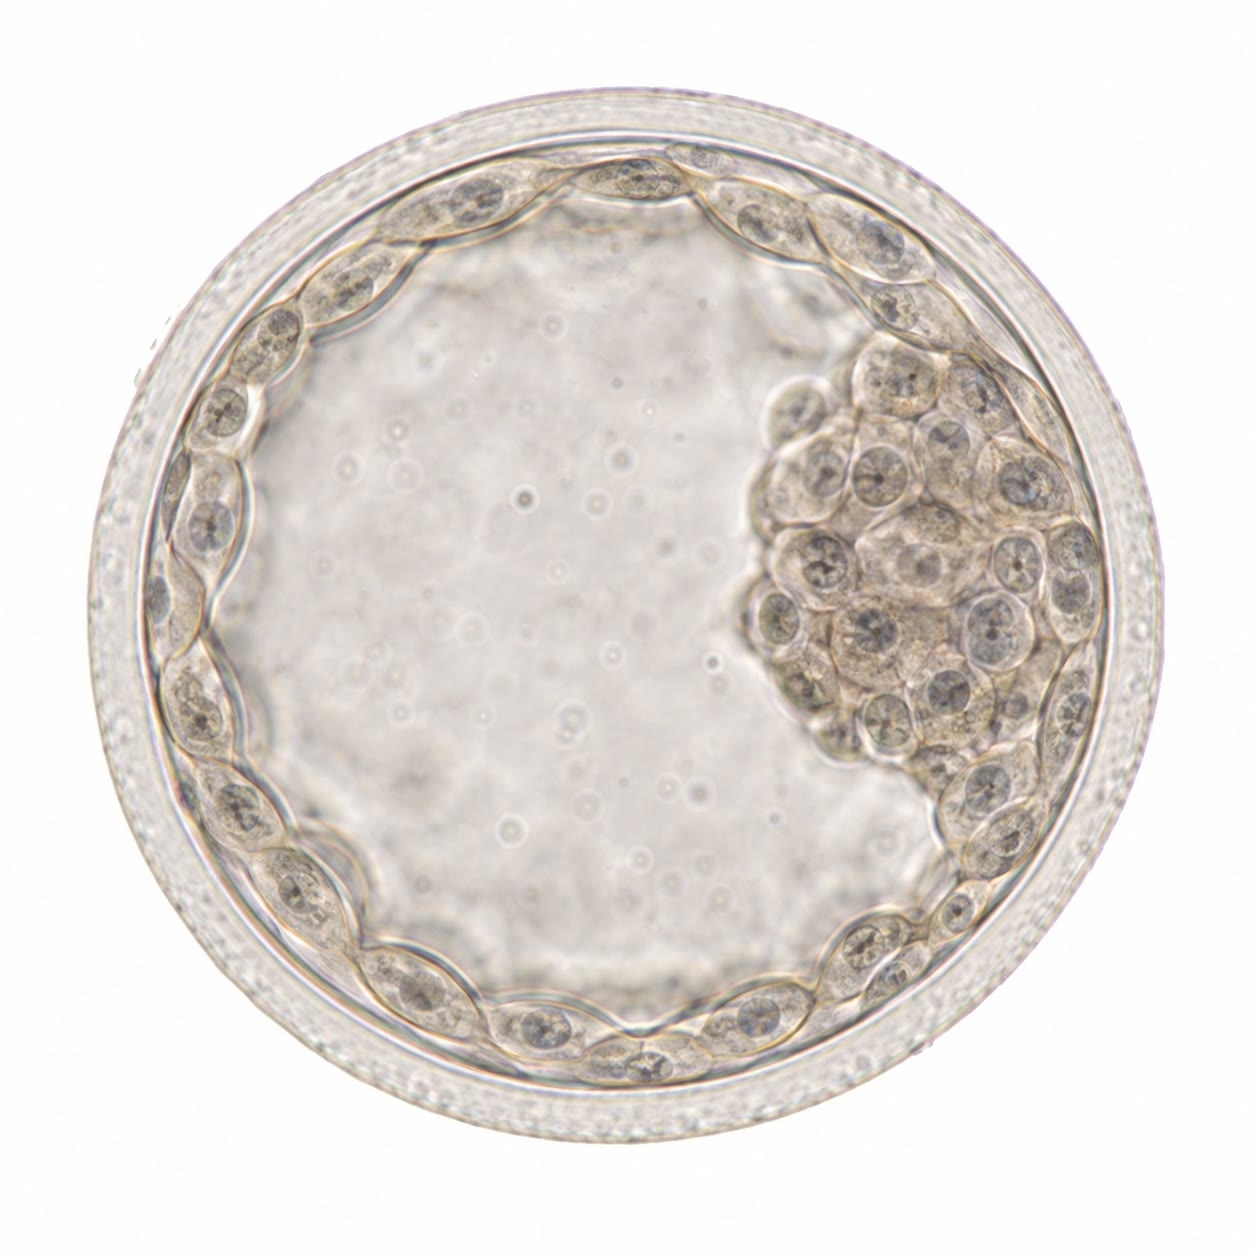
\includegraphics[width=0.42\linewidth]{images/book4/ai/b4-08-blastocyst.jpg}

{\small Een \omterm{def:b2:mammal-reproduction:implantation}{blastocyste} op dag vijf: de buitenste \omterm{def:b2:mammal-reproduction:implantation}{trofoblast} rond de
holte, en de \omterm{def:b2:mammal-reproduction:implantation}{binnenste celmassa} --- het toekomstige embryo --- aan één
kant.}
\end{omfigure}

\begin{definition}[De placenta]\label{def:b2:mammal-reproduction:placenta}
\index{placenta}\index{chorionvlok}\index{navelstreng}
De \emph{placenta} is een orgaan dat samen door het embryo (het chorion,
uit de \omterm{def:b2:mammal-reproduction:implantation}{trofoblast}) en de moeder (het baarmoederslijmvlies) wordt gemaakt.
Vingervormige \emph{chorionvlokken}, vertakt tot een oppervlak van zo'n
\qty{12}{m^2} aan het eind van de zwangerschap, hangen in meren van
maternaal bloed dat door de baarmoederslagaders met een halve liter per
minuut wordt aangevoerd; in elke vlok lopen foetale haarvaten, die via de
twee slagaders en de ene ader van de \emph{navelstreng} met de foetus zijn
verbonden. De twee bloedsoorten mengen nooit: ze zijn gescheiden door de
wand van de vlok, enkele micrometers \omterm{def:b2:mammal-reproduction:implantation}{trofoblast} en capillair endotheel,
waardoor zuurstof,
$\mathrm{CO_2}$, water, ureum en vetoplosbare moleculen diffunderen,
glucose en aminozuren door transporters worden gedragen, en maternale
antistoffen (IgG) via receptoren worden overgezet, wat de pasgeborene zijn
eerste maanden immuniteit geeft. De placenta is ook een klier: vanaf de
eerste dagen scheidt de \omterm{def:b2:mammal-reproduction:implantation}{trofoblast} \emph{humaan
choriongonadotrofine} (hCG) af, dat het \omterm{def:b2:mammal-reproduction:ovary}{corpus luteum} progesteron laat
blijven maken, en vanaf de derde maand maakt de placenta zelf het
progesteron en de oestrogenen die de zwangerschap in stand houden
(\cref{ch:b2:reproductive-hormones}). Ze is in feite een long, een darm,
een nier en een endocriene klier, gegroeid voor negen maanden en bij de
geboorte afgedankt.
\end{definition}

\begin{omfigure}
\begin{tikzpicture}[every node/.style={font=\scriptsize}, >=stealth]
  % maternal blood space
  \fill[omThm!12] (0,0) rectangle (8,3.6);
  \node[omThm!80!black, align=center] at (1.1,2.6) {maternaal bloed\\(intervilleuze\\ruimte)};
  % uterine wall at bottom
  \fill[omExo!30] (0,-0.6) rectangle (8,0); \node at (4,-0.3) {baarmoederwand (maternaal)};
  \draw[->, thick, omThm] (1.0,-0.6) -- (1.0,0.6); \node[omThm, anchor=west] at (1.05,0.3) {spiraalarterie};
  \draw[->, thick, omDef!60!black] (7.0,0.6) -- (7.0,-0.6); \node[omDef!60!black, anchor=east] at (6.95,0.3) {baarmoederader};
  % chorionic plate at top
  \fill[omDef!20] (0,3.6) rectangle (8,4.4); \node at (4,4.0) {chorionplaat (foetaal)};
  % villi hanging down
  \foreach \x in {2.6,4.2,5.8} {
    \draw[thick, fill=omDef!8] (\x-0.35,3.6) -- (\x-0.4,1.4) .. controls (\x-0.4,0.9) and (\x+0.4,0.9) .. (\x+0.4,1.4) -- (\x+0.35,3.6);
    \draw[thick, omThm!70!black] (\x-0.15,3.6) -- (\x-0.15,1.5) .. controls (\x-0.15,1.25) and (\x+0.15,1.25) .. (\x+0.15,1.5) -- (\x+0.15,3.6);
    \foreach \y in {2.0,2.7} { \draw[thick, fill=omDef!8] (\x-0.4,\y) .. controls (\x-0.9,\y+0.1) and (\x-0.9,\y-0.4) .. (\x-0.4,\y-0.3); }
  }
  % umbilical vessels
  \draw[very thick, omThm!70!black] (4.2,4.4) -- (4.2,5.0) node[above, align=center] {navelstrengader (naar de foetus)\\en slagaders};
  \draw[very thick, omDef!60!black] (3.9,4.4) -- (3.9,5.0); \draw[very thick, omDef!60!black] (4.5,4.4) -- (4.5,5.0);
  % exchange arrows
  \draw[<->, thick] (3.0,2.2) -- (3.75,2.2); \node[anchor=west, align=left] at (8.3,1.5) {door de wand: \textcolor{omThm}{O$_2$, glucose,}\\\textcolor{omThm}{aminozuren, IgG} naar de foetus;\\\textcolor{omDef!60!black}{CO$_2$, ureum} naar de moeder};
  \node[anchor=west, align=left] at (8.3,3.0) {wand van de vlok: trofoblast\\+ endotheel van de foetale haarvaten,\\enkele micrometers};
  \draw (6.2,2.5) -- (8.3,3.0);
\end{tikzpicture}

{\small De \omterm{def:b2:mammal-reproduction:placenta}{placenta}: foetale vlokken, die foetale haarvaten dragen, hangen
in een ruimte vol maternaal bloed uit de spiraalarteriën. De twee
bloedsoorten wisselen uit door de wand van de vlok en mengen nooit.}
\end{omfigure}

\begin{theorem}[Uitwisseling door de placenta]\label{thm:b2:mammal-reproduction:fick}
\index{wet van Fick!placenta}
Een gas dat een membraan met oppervlak $A$ en dikte $d$ passeert, beweegt
met een snelheid $J = K\,A\,\Delta P/d$, waarin $\Delta P$ het verschil in
zijn partiële druk is en $K$ de permeabiliteit van het weefsel. Voor
zuurstof in weefsel is $K \approx \qty{3e-8}{mL/(cm.min.mmHg)}$; met $A =
\qty{12}{m^2}$, $d = \qty{3.5}{\micro m}$ en $\Delta P =
\qty{20}{mmHg}$ (maternaal \qty{40}{mmHg} in de intervilleuze ruimte
tegen \qty{20}{mmHg} in de navelstrengslagader) zou de \omterm{def:b2:mammal-reproduction:placenta}{placenta} ongeveer
\qty{200}{mL} zuurstof per minuut kunnen doorlaten, zo'n acht keer de
\qty{25}{mL/min} die een voldragen foetus verbruikt. Het zuurstoftransport
wordt dus niet door diffusie beperkt maar door de bloedstroom; de foetus
werkt bij een lage zuurstofdruk en compenseert dat met een hemoglobine met
hogere affiniteit en een hoger aantal rode bloedcellen.
\end{theorem}
\begin{proof}
De wet van Fick stelt dat de flux evenredig is met de gradiënt
$\Delta P/d$ en met het oppervlak; de constante $K$ omvat de oplosbaarheid
en de diffusiecoëfficiënt van het gas in weefsel. Numeriek:
$3\times 10^{-8}\times 1.2\times 10^{5}\times 20/(3.5\times 10^{-4})
= \qty{206}{mL/min}$ met $A$ in \unit{cm^2} en $d$ in \unit{cm}.
De foetale behoefte is ongeveer \qty{7}{mL} per kilogram per minuut voor
\qty{3.5}{kg}.
\end{proof}

\section{Dracht, geboorte en lactatie}

\begin{proposition}[Dracht en geboorte]\label{prop:b2:mammal-reproduction:birth}
\index{dracht}\index{bevalling}\index{oxytocine}
De dracht duurt \num{20} dagen bij een muis, \num{280} bij een mens,
\num{660} bij een olifant --- ruwweg evenredig met de vierdemachtswortel
van de lichaamsmassa, waarbij primaten traag zijn voor hun grootte. Ze
wordt in stand gehouden door progesteron, dat de baarmoederspier rustig en
de baarmoederhals gesloten houdt. De geboorte (\emph{bevalling}) wordt door
de foetus zelf in gang gezet: zijn bijnierschorscortisol, dat aan het eind
van de zwangerschap stijgt, verschuift de \omterm{def:b2:mammal-reproduction:placenta}{placenta} van progesteron naar
oestrogeen, dat de baarmoeder uitrust met oxytocinereceptoren en gap
junctions en de afgifte van prostaglandinen op gang brengt. Dan neemt een
\emph{positieve terugkoppeling} het over: het hoofd drukt op de
baarmoederhals, sensorische zenuwen seinen de hypothalamus, \emph{oxytocine}
komt vrij uit de achterkwab van de hypofyse, de baarmoeder trekt samen, het
hoofd drukt harder; de lus escaleert tot de bevalling, waarna de prikkel
ophoudt en de lus stopt --- een van de weinige positieve terugkoppelingen
in de fysiologie, en een die in een gebeurtenis moet eindigen. De \omterm{def:b2:mammal-reproduction:placenta}{placenta}
volgt enkele minuten later.
\end{proposition}
\begin{proof}[Bewijsmateriaal]
Ferguson (1941) toonde bij het konijn aan dat het oprekken van de
baarmoederhals samentrekkingen van de baarmoeder uitlokte, en dat het
doorsnijden van het ruggenmerg of het verwijderen van de achterkwab van de
hypofyse de respons ophief: een neuro-endocriene reflex van baarmoederhals
via hypofyse naar baarmoeder. Oxytocine, in 1953 door du Vigneaud
geïsoleerd en gesynthetiseerd, is nu het standaardmiddel om de bevalling in
te leiden.
\end{proof}

\begin{proposition}[Lactatie]\label{prop:b2:mammal-reproduction:lactation}
\index{lactatie}\index{prolactine}\index{melk}
De melkklier, een gewijzigde zweetklier, wordt tijdens de zwangerschap
opgebouwd door oestrogeen, progesteron en prolactine, maar door progesteron
van secretie weerhouden; wanneer de \omterm{def:b2:mammal-reproduction:placenta}{placenta} vertrekt, daalt het
progesteron en beginnen de alveolen onder invloed van \emph{prolactine} uit
de voorkwab van de hypofyse melk te maken. Twee reflexen sturen het proces:
zogen stimuleert de afgifte van prolactine (die de synthese onderhoudt en
de \omterm{def:b2:mammal-reproduction:ovary}{ovulatie} onderdrukt) en van oxytocine (die de cellen rond de alveolen
laat samentrekken en de melk uitdrijft). Moedermelk bevat ongeveer
\qty{7}{\%} lactose, \qty{4}{\%} vet, \qty{1}{\%} eiwit en
\qty{2.9}{kJ/mL}; het \emph{colostrum} van de eerste dagen is rijk aan
antistoffen (IgA) die de darm van de zuigeling bekleden. Een moeder maakt
ongeveer \qty{750}{mL} per dag, tegen een kostprijs van zo'n \qty{2.5}{MJ}
--- een kwart van haar voedsel --- en dat maandenlang; lactatie is het
duurste deel van de voortplanting van zoogdieren, en het deel dat de
klasse haar naam geeft.
\end{proposition}

\section{De twee geslachten maken}

\begin{proposition}[Geslachtsbepaling en geslachtsdifferentiatie]\label{prop:b2:mammal-reproduction:sex}
\index{SRY}\index{anti-müllerhormoon}\index{geslachtsdifferentiatie}
Tot de zesde week heeft een menselijk embryo van beide geslachten dezelfde
uitrusting: een indifferente gonade, twee paar gangen (de \emph{gangen van
Wolff} en de \emph{gangen van Müller}) en neutrale uitwendige
geslachtsorganen. Het gen \emph{SRY} op het Y-chromosoom wordt in de gonade
aangeschakeld en maakt er een \omterm{def:b2:mammal-reproduction:testis}{testis} van; zonder dit gen wordt de gonade een
ovarium. De foetale \omterm{def:b2:mammal-reproduction:testis}{testis} doet dan twee dingen: zijn sertolicellen
scheiden het \emph{\omterm{prop:b2:mammal-reproduction:sex}{anti-müllerhormoon}} af, dat de gangen van Müller doet
verdwijnen, en zijn leydigcellen scheiden \emph{testosteron} af, dat de
gangen van Wolff behoudt (de latere bijbal, zaadleider en zaadblaasjes) en,
omgezet in dihydrotestosteron, de uitwendige geslachtsorganen vormt tot
penis en scrotum. Bij afwezigheid van beide signalen verdwijnen de gangen
van Wolff, worden de gangen van Müller de eileiders, de baarmoeder en het
bovenste deel van de vagina, en ontwikkelen de geslachtsorganen zich
vrouwelijk. De vrouwelijke weg is de weg die wordt ingeslagen wanneer er
niets wordt gezegd: de mannelijke weg moet door de \omterm{def:b2:mammal-reproduction:testis}{testis} actief worden
opgelegd, en elke stap waarop dat opleggen mislukt --- een mutant SRY, een
ontbrekende hormoonreceptor --- geeft een XY-individu met een vrouwelijk
of intermediair lichaam.
\end{proposition}
\begin{proof}[Bewijsmateriaal]
Jost (1947) verwijderde bij konijnenfoetussen in de baarmoeder de gonaden
voordat hun gangen gedifferentieerd waren: gecastreerde foetussen van
beide chromosomale geslachten ontwikkelden een baarmoeder, eileiders en
vrouwelijke geslachtsorganen. Een kristal testosteron dat in een
gecastreerde foetus werd ingeplant, behield aan die kant de gangen van
Wolff maar verwijderde de gangen van Müller niet; een getransplanteerde
foetale \omterm{def:b2:mammal-reproduction:testis}{testis} deed beide, aan zijn eigen kant: de \omterm{def:b2:mammal-reproduction:testis}{testis} moet een tweede,
toen onbekende factor maken om de vrouwelijke gangen te onderdrukken, die
dertig jaar later als \omterm{prop:b2:mammal-reproduction:sex}{anti-müllerhormoon} werd geïdentificeerd. Later bracht
het geslachtsomkerende effect van een klein stuk van het Y-chromosoom de
schakelaar terug tot \emph{SRY} (1990), en een muis die XX was gemaakt met
alleen het gen \emph{Sry}, ontwikkelde zich als mannetje.
\end{proof}

\begin{omfigure}
\begin{tikzpicture}[every node/.style={font=\scriptsize}, >=stealth]
  \node[draw, rounded corners, fill=omExo!25, align=center] (g) at (0,0) {indifferente gonade\\twee gangenstelsels};
  \node[draw, rounded corners, fill=omDef!15, align=center] (t) at (4.2,1.4) {testis\\(\emph{SRY} aanwezig)};
  \node[draw, rounded corners, fill=omThm!15, align=center] (o) at (4.2,-1.4) {ovarium\\(geen \emph{SRY})};
  \node[draw, rounded corners, fill=omDef!15, align=center] (amh) at (8.6,2.3) {AMH: gangen van Müller verdwijnen};
  \node[draw, rounded corners, fill=omDef!15, align=center] (tst) at (8.6,0.6) {testosteron: gangen van Wolff behouden;\\DHT: mannelijke uitwendige geslachtsorganen};
  \node[draw, rounded corners, fill=omThm!15, align=center] (f) at (8.6,-1.4) {geen signaal: gangen van Wolff verdwijnen,\\gangen van Müller $\to$ eileiders, baarmoeder;\\vrouwelijke geslachtsorganen};
  \draw[->, thick] (g) -- (t); \draw[->, thick] (g) -- (o);
  \draw[->, thick] (t) -- (amh); \draw[->, thick] (t) -- (tst); \draw[->, thick] (o) -- (f);
\end{tikzpicture}

{\small Geslachtsdifferentiatie: de \omterm{def:b2:mammal-reproduction:testis}{testis}, gemaakt door \emph{SRY}, legt met
twee hormonen de mannelijke weg op; bij hun afwezigheid ontwikkelt het
lichaam zich vrouwelijk.}
\end{omfigure}

\section{Opgaven}

\begin{exercise}[$\star$]\label{exo:b2:mammal-reproduction:1}
Vergelijk \omterm{def:b2:mammal-reproduction:testis}{spermatogenese} en \omterm{def:b2:mammal-reproduction:ovary}{oögenese}: wanneer de stamcellen zich delen,
hoeveel gameten één \omterm{def:b2:meiosis-heredity:meiosis}{meiose} oplevert, hoelang het maken van een gameet
duurt, waar de stilstanden liggen, en hoeveel gameten een leven
voortbrengt.
\end{exercise}

\begin{exercise}[$\star$]\label{exo:b2:mammal-reproduction:2}
Noem de stappen van de bevruchting van de aankomst van een zaadcel bij de
zona tot de eerste mitose, en zeg welke stap polyspermie blokkeert.
\end{exercise}

\begin{exercise}[$\star$]\label{exo:b2:mammal-reproduction:3}
Noem de twee celpopulaties van de \omterm{def:b2:mammal-reproduction:implantation}{blastocyste} en het lot van elk. Op welke
dag begint de \omterm{def:b2:mammal-reproduction:implantation}{innesteling}, en welk hormoon moet de baarmoeder hebben
voorbereid?
\end{exercise}

\begin{exercise}[$\star$]\label{exo:b2:mammal-reproduction:4}
Zeg van elk van de volgende of het de \omterm{def:b2:mammal-reproduction:placenta}{placenta} passeert, en hoe: zuurstof,
glucose, maternale rode bloedcellen, IgG-antistoffen, ureum, alcohol, de
meeste bacteriën.
\end{exercise}

\begin{exercise}[$\star\star$]\label{exo:b2:mammal-reproduction:5}
Bereken met $\pi = 10^{-8}$ per zaadcel de kans op bevruchting bij
aantallen zaadcellen van $3\times 10^{8}$, $10^{8}$,
$4\times 10^{7}$ en $10^{7}$. Bij welk aantal zakt ze onder de helft? Wat
zegt dit over de vorm van de dosis-responsrelatie tussen vruchtbaarheid en
aantal zaadcellen?
\end{exercise}

\begin{exercise}[$\star\star$]\label{exo:b2:mammal-reproduction:6}
Een meisje wordt geboren met $10^{6}$ oöcyten, heeft er \num{300000} bij
de puberteit (13 jaar) en ongeveer \num{1000} op 50 jaar, na er \num{400}
te hebben geovuleerd. Bereken het gemiddelde tempo van atresie (verloren
oöcyten per dag) vóór en na de puberteit, en vergelijk met het tempo van
\omterm{def:b2:mammal-reproduction:ovary}{ovulatie}.
\end{exercise}

\begin{exercise}[$\star\star$]\label{exo:b2:mammal-reproduction:7}
Foetaal hemoglobine heeft een halfverzadigingsdruk $P_{50} =
\qty{19}{mmHg}$, volwassen hemoglobine \qty{27}{mmHg}; neem voor de
verzadiging $S = P^{n}/(P_{50}^{n} + P^{n})$ met $n = 2.7$.
Bereken beide verzadigingen bij \qty{30}{mmHg}, de druk in de
navelstrengader, en leg het voordeel uit.
\end{exercise}

\begin{exercise}[$\star\star$]\label{exo:b2:mammal-reproduction:8}
hCG verschijnt bij de \omterm{def:b2:mammal-reproduction:implantation}{innesteling} (dag 7 na de bevruchting) in het
maternale bloed met ongeveer \qty{1}{IU/L} en verdubbelt om de twee dagen;
een zwangerschapstest detecteert \qty{25}{IU/L}. Op welke dag na de
bevruchting wordt de test positief? Op welke dag na de laatste menstruatie
(\omterm{def:b2:mammal-reproduction:ovary}{ovulatie} op dag 14)?
\end{exercise}

\begin{exercise}[$\star\star$]\label{exo:b2:mammal-reproduction:9}
Bereken het zuurstoftransport door de \omterm{def:b2:mammal-reproduction:placenta}{placenta} uit de stelling opnieuw voor
een \omterm{def:b2:mammal-reproduction:placenta}{placenta} van \qty{6}{m^2} met een vlokwand van \qty{10}{\micro m}, zoals
bij sommige aandoeningen, en vergelijk met de foetale behoefte. Wat gebeurt
er met de foetus?
\end{exercise}

\begin{exercise}[$\star\star\star$]\label{exo:b2:mammal-reproduction:10}
Voorspel het gangenstelsel en de uitwendige geslachtsorganen van: (a) een
XY-foetus waarvan de cellen de testosteronreceptor missen; (b) een
XY-foetus zonder \omterm{prop:b2:mammal-reproduction:sex}{anti-müllerhormoon}; (c) een XX-foetus die aan hoge
testosteronspiegels uit zijn bijnieren is blootgesteld; (d) een XX-foetus
die \emph{SRY} op een X-chromosoom draagt. Verklaar elk geval met de
resultaten van Jost.
\end{exercise}

\begin{exercise}[$\star\star\star$]\label{exo:b2:mammal-reproduction:11}
Eeneiige tweelingen ontstaan wanneer één embryo zich splitst. Splitst het
vóór dag 3, dan hebben de tweelingen aparte \omterm{def:b2:mammal-reproduction:placenta}{placenta}'s en vruchtzakken;
tussen dag 4 en 8 één \omterm{def:b2:mammal-reproduction:placenta}{placenta} en twee vruchtzakken; tussen dag 8 en 13
één \omterm{def:b2:mammal-reproduction:placenta}{placenta} en één vruchtzak; later zijn ze vergroeid. In een reeks
eeneiige tweelingen heeft \qty{30}{\%} aparte \omterm{def:b2:mammal-reproduction:placenta}{placenta}'s, \qty{68}{\%} één
\omterm{def:b2:mammal-reproduction:placenta}{placenta} en twee vruchtzakken, \qty{2}{\%} één vruchtzak. Leid af in welk
ontwikkelingsstadium de splitsing het vaakst plaatsvindt, en leg aan de
hand van de \omterm{def:b2:mammal-reproduction:implantation}{blastocyste} uit welke structuren in elk geval worden gedeeld.
\end{exercise}

\begin{exercise}[$\star\star\star$]\label{exo:b2:mammal-reproduction:12}
Buideldieren baren na enkele weken een jong zo groot als een boon, dat
zijn groei aan een tepel in de buidel voltooit; placentale zoogdieren
dragen lang en baren een groot jong. Vergelijk de twee strategieën in
termen van kosten voor de moeder, risico, en het vermogen van de moeder om
in een slecht seizoen een worp op te geven, en suggereer waarom placentale
zoogdieren de buideldieren op elk continent behalve Australië hebben
verdrongen.
\end{exercise}

\section{Vraagstuk: een zwangerschap in getallen}

\begin{problem}[{Weekendvraagstuk --- een menselijke zwangerschap gevolgd
van de zaadcel tot de melk, via de kansen op bevruchting, het tijdstip van
de innesteling en haar hormoon, de uitwisselingscapaciteit van de placenta
en de energiekosten van dracht en lactatie, met als besluit de kans op
bevruchting, de dag waarop de test positief wordt, de zuurstofmarge van de
placenta en de kosten van een dag melk}]
\label{pb:b2:mammal-reproduction:1}
Gegevens: $3\times 10^{8}$ zaadcellen per zaadlozing, die elk met kans
$10^{-8}$ de eicel bereiken; zaadcellen zwemmen met \qty{50}{\micro m/s};
de ampulla ligt op \qty{15}{cm} van de baarmoederhals. hCG bij de
\omterm{def:b2:mammal-reproduction:implantation}{innesteling} (dag 7) \qty{1}{IU/L}, verdubbelend om de \qty{2}{d},
testdrempel \qty{25}{IU/L}. \omterm{def:b2:mammal-reproduction:placenta}{Placenta} aan het eind van de zwangerschap:
\qty{12}{m^2}, wand
\qty{3.5}{\micro m}, $K_{\mathrm{O_2}} = \qty{3e-8}{mL/(cm.min.mmHg)}$,
$\Delta P = \qty{20}{mmHg}$; foetus van \qty{3.5}{kg} die
\qty{7}{mL} zuurstof per kilogram per minuut verbruikt; maternale
placentaire bloedstroom \qty{500}{mL/min} met \qty{0.16}{mL} zuurstof per
milliliter bloed. Glucose: de foetus gebruikt \qty{5}{mg} per kilogram per
minuut; maternaal bloed \qty{0.9}{g/L}. Melk: \qty{750}{mL/d} met
\qty{2.9}{kJ/mL}, gemaakt met een rendement van \qty{80}{\%}; de zuigeling
groeit \qty{30}{g/d} aan weefsel met \qty{6}{kJ/g} afgezet en besteedt
\qty{300}{kJ/kg/d} aan onderhoud bij \qty{4}{kg}.

\medskip
\noindent\textbf{Deel I --- Bevruchting.}
\begin{enumerate}
  \item Bereken het gemiddelde aantal zaadcellen dat de eicel bereikt en de
        kans op bevruchting.
  \item Bereken de kans dat er twee of meer aankomen, en zeg wat er zonder
        de \omterm{prop:b2:mammal-reproduction:fertilisation}{corticale reactie} zou gebeuren.
  \item Hoelang zou een zaadcel erover doen om naar de ampulla te zwemmen?
        Men vindt er binnen \qty{30}{min} zaadcellen: wat voert ze mee?
  \item Slechts enkele honderden zaadcellen bereiken de ampulla. Welk deel
        van de zaadlozing is dat, en waar gaan de andere verloren?
  \item Een eicel is ongeveer een dag bevruchtbaar, zaadcellen overleven
        ongeveer drie dagen in het vrouwelijke kanaal. Over hoeveel dagen van
        de cyclus kan geslachtsgemeenschap tot conceptie leiden?
  \item Het aantal zaadcellen van een man daalt tot $5\times 10^{7}$.
        Bereken opnieuw de kans op bevruchting per cyclus, en het verwachte
        aantal cycli tot conceptie (geometrische verdeling).
  \item Leg uit waarom de eicel, en niet de zaadcel, de mitochondriën van
        het embryo levert.
\end{enumerate}

\medskip
\noindent\textbf{Deel II --- De \omterm{def:b2:mammal-reproduction:implantation}{innesteling} en haar hormoon.}
\begin{enumerate}[resume]
  \item Hoeveel klievingsdelingen hebben er tegen dag 5 plaatsgevonden als
        ze elk \qty{16}{h} duren? Hoeveel cellen?
  \item Op welke dag na de bevruchting bereikt hCG de testdrempel? Na de
        laatste menstruatie (\omterm{def:b2:mammal-reproduction:ovary}{ovulatie} op dag 14)?
  \item Waarom moet hCG binnen enkele dagen na de \omterm{def:b2:mammal-reproduction:implantation}{innesteling} verschijnen?
        Wat gebeurt er met het \omterm{def:b2:mammal-reproduction:ovary}{corpus luteum}, en met de zwangerschap, als
        dat niet zo is?
  \item hCG piekt rond week 10 bij ongeveer \qty{1e5}{IU/L} en daalt
        daarna. Hoeveel verdubbelingen vanaf de \omterm{def:b2:mammal-reproduction:implantation}{innesteling} zijn dat, en
        waarom kan het daarna dalen zonder dat de zwangerschap verloren
        gaat?
  \item De helft van de conceptussen gaat vóór of bij de \omterm{def:b2:mammal-reproduction:implantation}{innesteling}
        verloren, meestal door aneuploïde eicellen. Leg met de tijdlijn van
        de \omterm{def:b2:mammal-reproduction:ovary}{oögenese} uit waarom aneuploïdie vaker voorkomt bij eicellen dan
        bij zaadcellen.
  \item Tweelingen: een embryo dat zich op dag 6 splitst. Zeg of de
        tweelingen de \omterm{def:b2:mammal-reproduction:placenta}{placenta} en de vruchtzak delen.
\end{enumerate}

\medskip
\noindent\textbf{Deel III --- De \omterm{def:b2:mammal-reproduction:placenta}{placenta}.}
\begin{enumerate}[resume]
  \item Bereken het maximale diffusieve zuurstoftransport.
  \item Bereken de zuurstofbehoefte van de foetus en de diffusiemarge.
  \item Bereken de zuurstof die de maternale bloedstroom per minuut aan de
        \omterm{def:b2:mammal-reproduction:placenta}{placenta} levert. Welke fractie moet worden onttrokken om aan de
        behoefte te voldoen?
  \item Bereken de glucosebehoefte van de foetus in gram per dag, en het
        volume maternaal bloed dat die bevat. Vergelijk met de dagelijkse
        maternale placentaire bloedstroom.
  \item Het bloed van de foetus verlaat de \omterm{def:b2:mammal-reproduction:placenta}{placenta} met \qty{30}{mmHg}
        zuurstof. Waarom stikt de foetus niet bij een druk die een
        volwassene bewusteloos zou maken?
  \item Noem twee dingen die de \omterm{def:b2:mammal-reproduction:placenta}{placenta} doet en die geen ander orgaan van
        het embryo op dat moment kan doen, en één ding dat ze niet kan.
\end{enumerate}

\medskip
\noindent\textbf{Deel IV --- Geboorte en melk.}
\begin{enumerate}[resume]
  \item Beschrijf de positieve terugkoppeling van de bevalling en leg uit
        waarom ze vóór het einde van de zwangerschap niet op hol slaat.
  \item Bereken de energie in de melk van een dag en de energie die de
        moeder besteedt om die te maken.
  \item Bereken het dagelijkse energiebudget van de zuigeling (groei plus
        onderhoud) en vergelijk met de geleverde melk.
  \item Bereken de totale energiekosten voor de moeder van negen maanden
        lactatie, en vergelijk met de \qty{300}{MJ} die de zwangerschap zelf
        kost.
  \item Leg uit waarom zogen de terugkeer van de \omterm{def:b2:mammal-reproduction:ovary}{ovulatie} uitstelt, en
        waarom dit van belang is in populaties zonder anticonceptie.
  \item Formuleer het resultaat: de kans op bevruchting, de dag waarop de
        test positief wordt, de zuurstofmarge van de \omterm{def:b2:mammal-reproduction:placenta}{placenta}, en de
        kosten van een dag melk.
\end{enumerate}
\end{problem}
